%%%%%%%%%%%%%%%%%%%%%%%%%%%%%%%%%%%%%%%%%
% a0poster Portrait Poster
% LaTeX Template
% Version 1.0 (22/06/13)
%
% The a0poster class was created by:
% Gerlinde Kettl and Matthias Weiser (tex@kettl.de)
% 
% This template has been downloaded from:
% http://www.LaTeXTemplates.com
%
% License:
% CC BY-NC-SA 3.0 (http://creativecommons.org/licenses/by-nc-sa/3.0/)
%
%%%%%%%%%%%%%%%%%%%%%%%%%%%%%%%%%%%%%%%%%

%----------------------------------------------------------------------------------------
%	PACKAGES AND OTHER DOCUMENT CONFIGURATIONS
%----------------------------------------------------------------------------------------

\documentclass[a0,portrait]{a0poster}

\usepackage{multicol} % This is so we can have multiple columns of text side-by-side
\columnsep=100pt % This is the amount of white space between the columns in the poster
\columnseprule=3pt % This is the thickness of the black line between the columns in the poster
%\usepackage[,activeacute]{babel}
%\usepackage{babelbib}
\usepackage{natbib}
\usepackage[svgnames]{xcolor} % Specify colors by their 'svgnames', for a full list of all colors available see here: http://www.latextemplates.com/svgnames-colors
\usepackage{times} % Use the times font
%\usepackage{palatino} % Uncomment to use the Palatino font
\usepackage{amsmath}
\usepackage{graphicx} % Required for including images
%\graphicspath{{figures/}} % Location of the graphics files
\usepackage{booktabs} % Top and bottom rules for table
\usepackage[font=small,labelfont=bf]{caption} % Required for specifying captions to tables and figures
\usepackage{amsfonts, amsmath, amsthm, amssymb} % For math fonts, symbols and environments
\usepackage{wrapfig} % Allows wrapping text around tables and figures
\usepackage{comment}
\usepackage{multicol}
\usepackage{MnSymbol,wasysym}

\usepackage[T1]{fontenc}
\usepackage[sfdefault]{AlegreyaSans} %% Option 'black' gives heavier bold face



\newcommand{\minx}{0}
\newcommand{\maxx}{\infty}
\newcommand{\minpar}{0}
\newcommand{\maxpar}{\infty}
\newcommand{\comire}{\textsc{c}o\textsc{m}i\textsc{r}e }
\newcommand{\comirep}{\textsc{c}o\textsc{m}i\textsc{r}e}

\graphicspath{{./figures/}}

\RequirePackage{import}
\RequirePackage{bm}
\RequirePackage{pdfpages}
\RequirePackage{transparent}
\RequirePackage{xcolor}
\newcommand{\incfig}[2][1]{%
    \def\svgwidth{#1\textwidth}
    \import{./figures/}{#2.pdf_tex}
}

\usepackage{statmacros}
\usepackage{useful-packages}
\begin{document}

%----------------------------------------------------------------------------------------
%	POSTER HEADER 
%----------------------------------------------------------------------------------------

% The header is divided into two boxes:
% The first is 75% wide and houses the title, subtitle, names, university/organization and contact information
% The second is 25% wide and houses a logo for your university/organization or a photo of you
% The widths of these boxes can be easily edited to accommodate your content as you see fit

\begin{minipage}[c]{0.75\linewidth}
\huge \color{DarkRed} \textbf{Bayesian nonparametric multiscale mixture models via Hilbert-curve partitioning}\\[0.5cm]  \color{Black} % Title
%\Huge\textit{Prueba de Relatividad General a Grandes Escalas}\\[2cm] % Subtitle
\huge \textbf{Daniele Zago}\\[0.5cm] % Author(s)
\Large Department of Statistical Sciences, University of Padova \\[0.5cm]
\large
Joint work with Antonio Canale,  University of Padova \& Marco Stefanucci, Sapienza Università di Roma
%\Large \texttt{Grupo 8330, Semestre 2016-I} --- Cosmolog\'ia Observacional\\
\end{minipage}
%
\begin{minipage}[c]{0.25\linewidth}

\includegraphics[scale=0.2]{logo_unipd}
\end{minipage}

\vspace{1cm} % A bit of extra whitespace between the header and poster content

%----------------------------------------------------------------------------------------

\begin{multicols}{2} % This is how many columns your poster will be broken into, a portrait poster is generally split into 2 columns

%----------------------------------------------------------------------------------------
%	ABSTRACT
%----------------------------------------------------------------------------------------

\color{DarkRed}

\section*{Abstract}

\begin{itemize}
\item[] We consider the problem of flexible \textbf{nonparametric density estimation} using mixtures of densities.
\item[] We are motivated by \textbf{astrological applications}, where galaxies might be clustered based on their colour spectrum.
% \item[] We want to define a model that is {\bf flexible} and {\bf parsimonious}, and {\bf interpretable}.
\item[] We rely on a \textbf{multiscale mixture model for the density} in order to \textbf{cluster observations at different resolutions}
\item[] The multiscale structure is described by using a \textbf{sequence of Hilbert curves} in order to \textbf{map the multivariate space to a binary tree}
\item[] The resulting mixture is \textbf{flexible} and can \textbf{adapt} very well \textbf{to the underlying smoothness} of the data
% \item[] The resulting {\bf Bayesian convex mixture regression (\comirep)} model allows the entire distribution of $y$ to be unknown and changing flexibly with $x$ and provides a more parsimonious, but still powerful, formulation compared to standard nonparametric methods
\end{itemize}

%----------------------------------------------------------------------------------------
%	INTRODUCTION
%----------------------------------------------------------------------------------------


\section*{Motivating application}
\color{Black}
\begin{itemize}
\item[] We focus on relating {\bf \textsc{dde} exposure}, henceforth $x$, in pregnant women to the risk of a {\bf premature delivery} (Longnecker et al., 2001)
\item[] The data set is obtained from a sub-study of the US Collaborative Perinatal Project (CPP) 
\item[] The values of $x$ are measured in $n$ pregnant women and $y$ is their gestational age at delivery
\item[] Figure 1 shows the histogram of $y$ for interval of $x$ {\color{blue} (warning: spoiler ahead!)}
\end{itemize}


%\begin{figure} 
%\centering
 %  \caption{The figure appears in color in the electronic version of this article.}
  % \label{fig:motivate}
%\end{figure}

% \begin{figure}[htbp]
%     \centering
%     % trim l b r u
%     \input{figures/bintree.pdf_tex}
%     \caption{Binary tree representation of the mixture model, truncated at scale $s = 3$. At each node, $\bm{\vartheta}_{s,h}$ and $\pi_{s,h}$ are the associated kernel parameters and mixture weight, respectively.}
%     \label{fig:btree}
% \end{figure}

\begin{itemize}
\item[] In quantitative risk assessment we are interested in quantifying {\bf risk} (Piegorsch and Bailer, 2005)
\item[] Risk is defined by the additional {\bf risk function }(Kodell and West, 1993), i.e.
\begin{eqnarray*} 
R_{\mbox{\textsc{a}}}(x,a) &=&  \mbox{pr}(y \leq a \mid x)- \mbox{pr}(y \leq a \mid x=0)=F_x(a)-F_0(a)
\label{add_risk}
\end{eqnarray*}
\item[] In the above equation $a$ corresponds to a threshold of clinical interest (e.g. $a=37$ weeks, for premature delivery)
\end{itemize}

\color{DarkRed}
\section*{Background}
\color{Black}

\subsection*{Multiscale models}
\color{Black}

\begin{itemize}
    \item[] Multiscale model define a mixture of increasingly concentrated kernels, e.g.

        \[
            f(y) = \sum_{s=0}^{\infty }\sum_{h=1}^{2^{s}} \pi_{s,h} \mathcal{K}(y; \bm{\mu}_{s,h}, \Omega_{s,h}),
        \]

        where $(s,h)$ \textbf{corresponds to a node of a binary tree} and $ \mathcal{K}$ is a multivariate scale and location kernel.
        
    \item[] $ \mathcal{K}$ is \textbf{increasingly concentrated} as $ s$ increases, and the location parameter $ \bm{\mu}_{s,h}$ should \textbf{span the whole space} as $ h$ moves between the values $ 1, \ldots, 2^{s}$.

    \item[] The nonparametric prior distribution for the mixture weights $ \pi_{s,h}$ has been developed by \citet{canale2016b}
        
\end{itemize}


\color{Black}
\begin{center}\vspace{1cm}
  \input{figures/bintree.pdf_tex}
  \captionof{figure}{}
\end{center}\vspace{1cm}

\begin{flushright}
    \color{ForestGreen}
    \smiley{} Pro: flexibility and adaptability to data smoothness

\noindent
\color{red}
\frownie{} Con: Hard to generalize the binary tree to multivariate mixtures
\end{flushright}

%----------------------------------------------------------------------------------------
%	OBJECTIVES
%----------------------------------------------------------------------------------------

\color{DarkRed}
\section*{Solution: use Hilbert curve partitioning}
\color{Black}

    We partition the location space $ \Theta_{\bm{\mu}}$ so that we span the whole space in $ h$ and the partitions are nested,
        \[
            \Theta_{\bm{\mu}} = \bigcup_{h=1}^{2^{s}} \Theta_{\bm{\mu}; s,h}, \quad  \Theta_{\bm{\mu}; s,h} = \Theta_{\bm{\mu}; s+1, 2h-1} \cup \Theta_{\bm{\mu};s+1, 2h}.
        \]

\vspace{.5cm}

The partition is done using the following two-stage procedure:
\begin{enumerate}
    \item Partition the cube $ [0,1]^{d}$ using the Hilbert curve (Figure~\ref{fig:partition-2d}).

    \item Apply conditional quantiles of $ G_0$ to the extremes of each subcube.
\end{enumerate}

\begin{center}
    % trim l b r u
    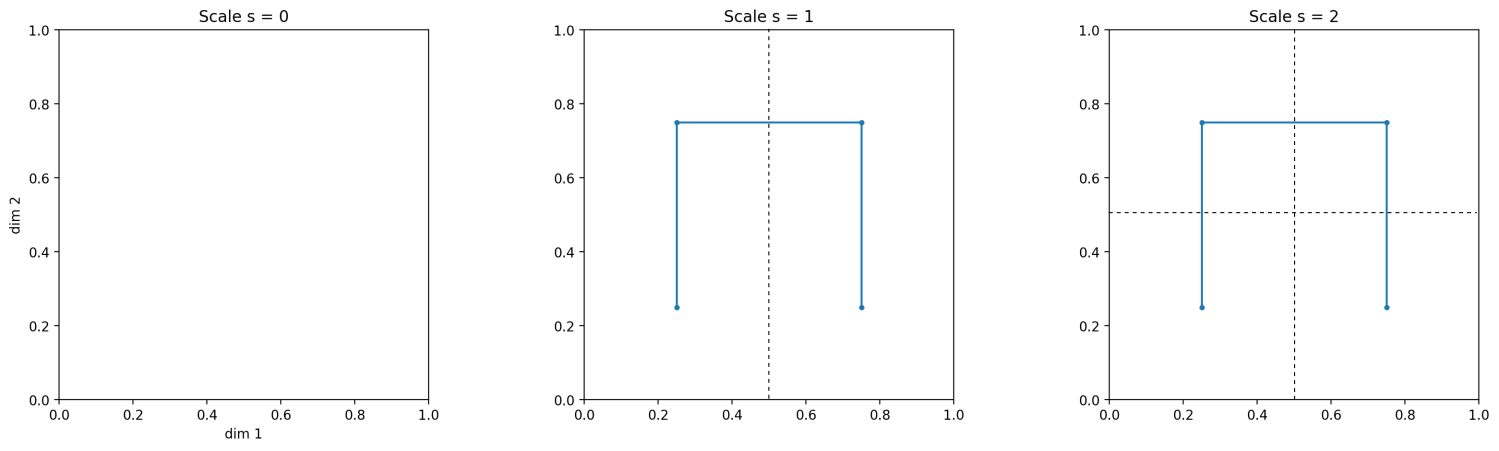
\includegraphics[trim={0 0 0 0}, clip, width=0.45\textwidth]{figures/partition_2d_top2.png}
    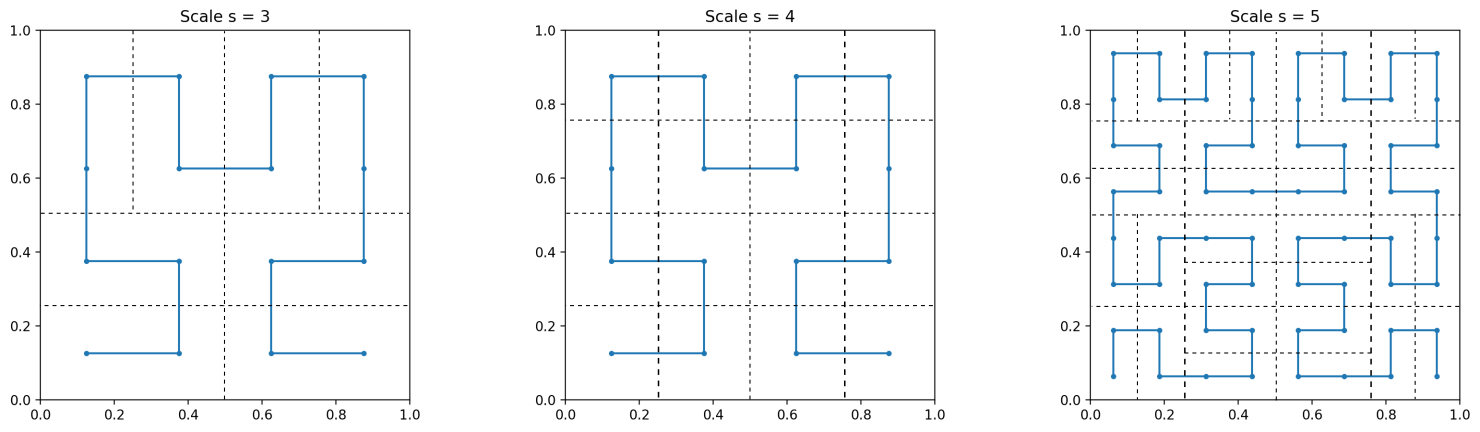
\includegraphics[trim={0 0 0 0}, clip, width=0.45\textwidth]{figures/partition_2d_bot2.png}
    \captionof{figure}{Dyadic partition of $[0,1]^2 $ obtained by the application of the Hilbert curve, for $ s = 1, \ldots, 5$.
    }
    \label{fig:partition-2d}
\end{center}

Sampling at each node from $ G_0$ truncated to $ \Theta_{\bm{\mu}; s,h}$ yields the \textbf{prior for the location parameter}, whereas $ \Omega_{s,h}$ are sampled from a distribution $ H_0$ \textbf{scaled by a deterministic monotone decreasing sequence} in $ s$.
%##########################################################
\color{DarkRed}
\section*{Interpretation}
\label{prop}
\color{Black}
%##########################################################

\begin{itemize}
\item Nodes higher in the tree correspond to \textbf{coarser kernels} whereas deeper nodes correspond to more \textbf{localized kernels}.
    The posterior adapts the kernels to the smoothness of the data.
\item We show that the random \textit{a priori} location measure $G = \sum_{s=0}^{\infty }\sum_{h=1}^{2^s} \pi_{s,h} \delta_{\bm{\mu}_{s,h}}$ is \textbf{centered around $ G_0$},
    \[
        \mathbb{E}[G(A)] = G_0(A)\quad \text{for all $ A \subseteq \Theta_{\bm{\mu}}$}.
    \]
    

\end{itemize}
\color{DarkRed}
\vspace{-0.3cm}

\color{DarkRed}
\section*{Performance in simulated datasets}
\color{Black}
\begin{itemize}
\item Scenarios: 1) correctly specified, 2) misspecified ---\textsc{ddp}, 3) misspecified ---no $x$ effect
\item Competitors: {\color{blue} \comirep}, {\color{red}\textsc{ddp}} \citep{deio:etal}, {\color{green} probit stick-breaking} \citep{rodriguez:2011}
\item Inference on true additional risk function  $R_{\mbox{\textsc{a}}}(x,37)$ (shaded areas 95\% credible bands) in Figure 2
\end{itemize}

 \begin{center}\vspace{1cm}
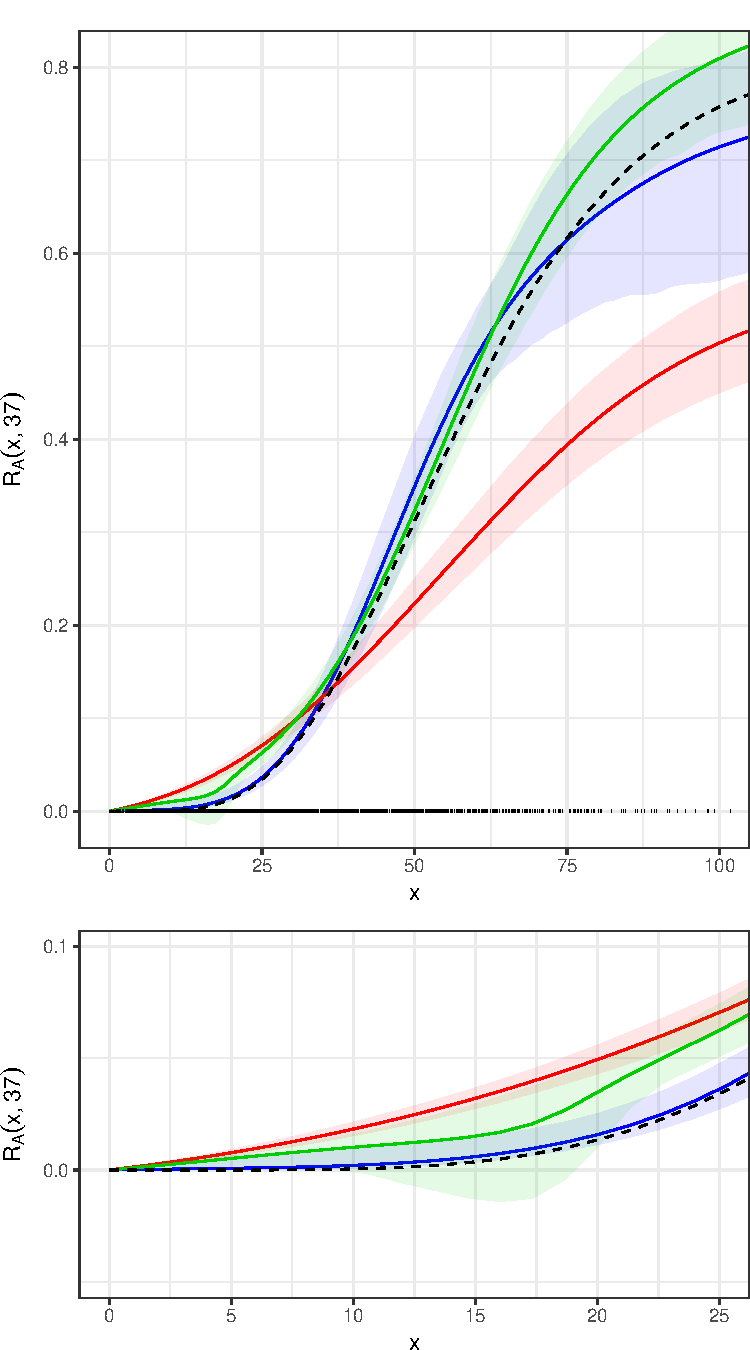
\includegraphics[width=0.15\textwidth]{risk1_37}
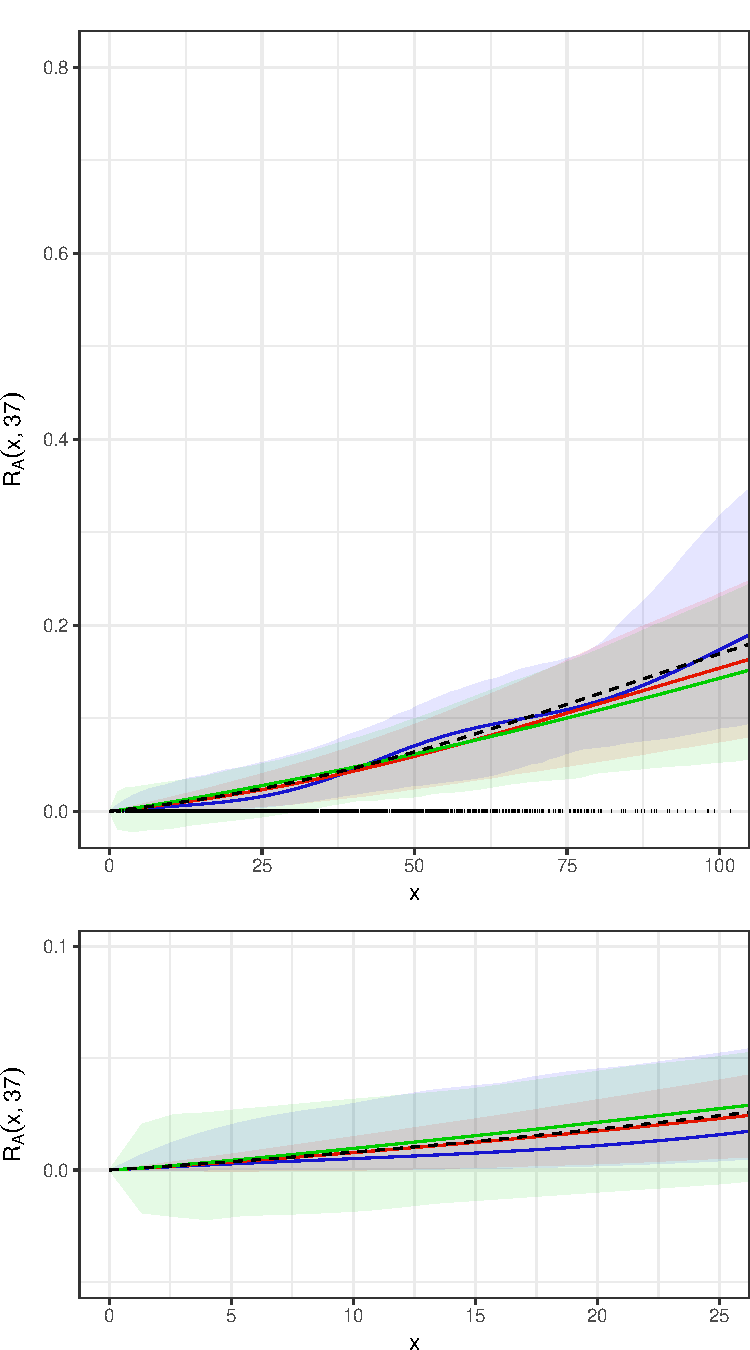
\includegraphics[width=0.15\textwidth]{risk2_37}
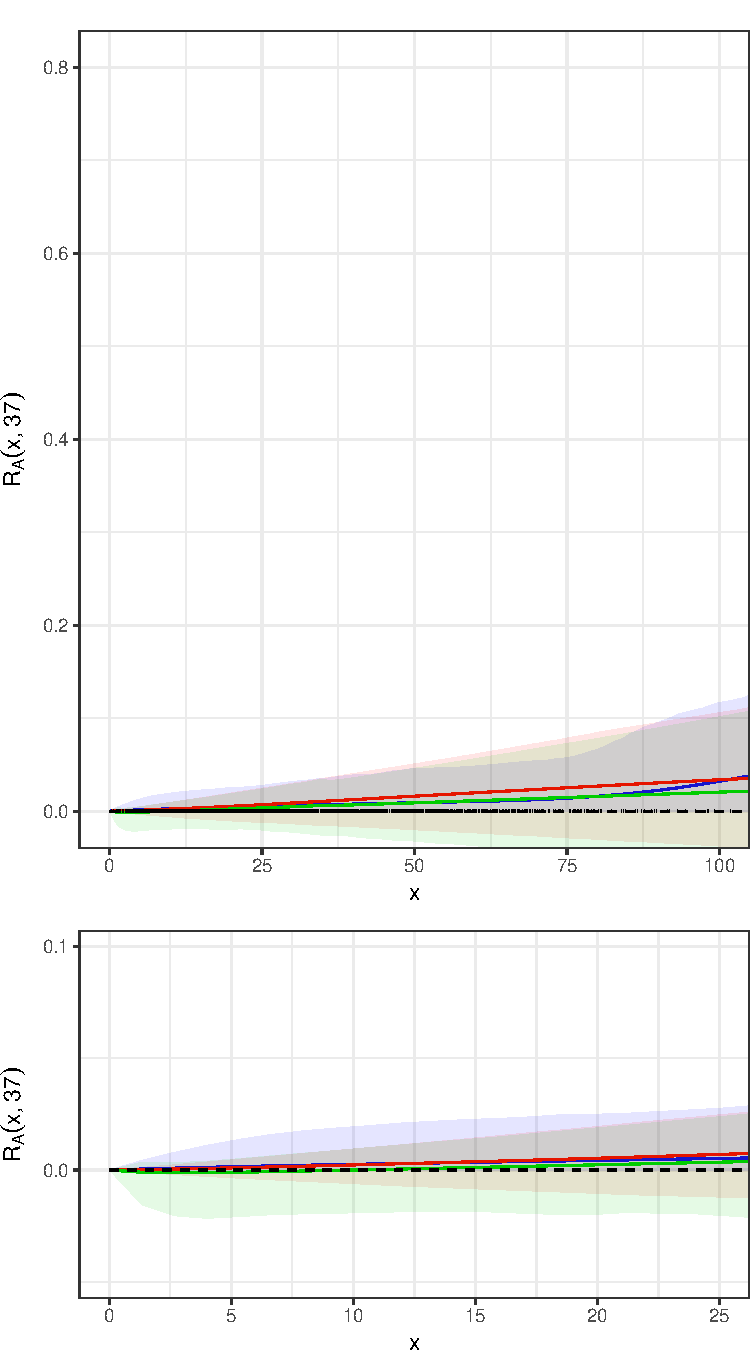
\includegraphics[width=0.15\textwidth]{risk3_37}
\captionof{figure}{Inference on the additional risk function for the three scenarios.}
\end{center}

\vspace{-0.5cm}

%##############-####################################################
\color{DarkRed}
\section*{Analysis of the CPP Data}
\label{cpp}
\color{Black}

%##############-####################################################

\begin{itemize}
\item According to Figure~1, the conditional density of the  gestational age at delivery is far from being Gaussian and displays variability, skewness, and multimodality 
\item at low--doses, the probability mass is concentrated around normal pregnancies, with the posterior mean (and 95\% c.i.) for $\mu(0)$ being $40.20$  $(40.01,40.34)$
\item as \textsc{dde} grows the negative skewness is still maintained, and preterm deliveries increasingly inflates
\item for {\bf benchmark dose analyses} the posterior mean and the $95\%$ c.i. of the BMD$_q$ are reported in Figure~3.
\end{itemize}


%
\begin{minipage}{0.15\textwidth}
\begin{tabular}{lrrr}
 \multicolumn{4}{c}{Benchmark doses $q$}\\
    \hline
  $q$& {\bf 0.01} & {\bf 0.05} & {\bf 0.10}  \\ 
  \hline
 BMD$_q$ & 1.03  & 5.79 & 15.29 \\ 
 BMDL$_q$ & 0.64 & 3.70 & 9.85 \\
   \hline
\end{tabular}
\end{minipage}
%
\begin{minipage}[c]{0.15\textwidth}
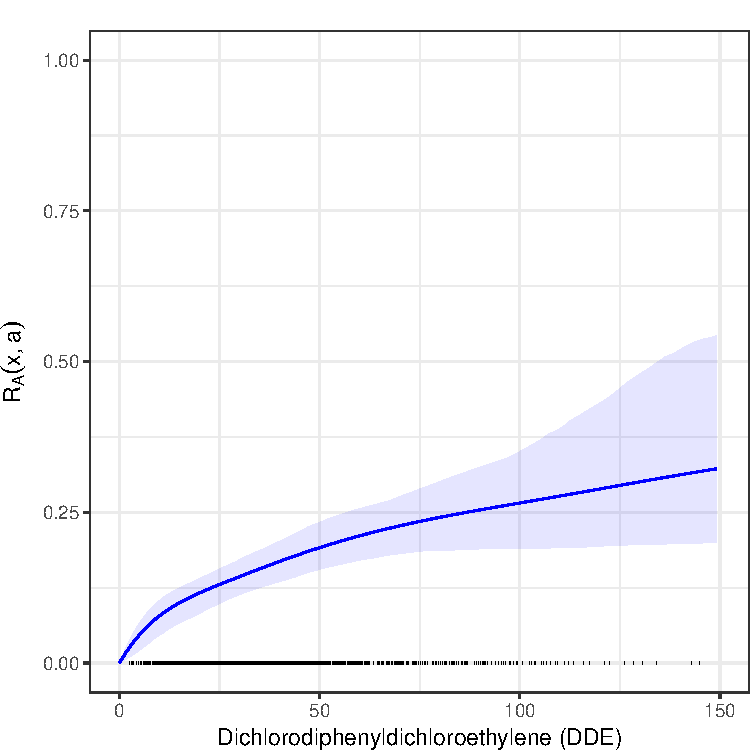
\includegraphics[width=1\textwidth]{cpp_risk}
\end{minipage}
%
\begin{minipage}[c]{0.15\textwidth}
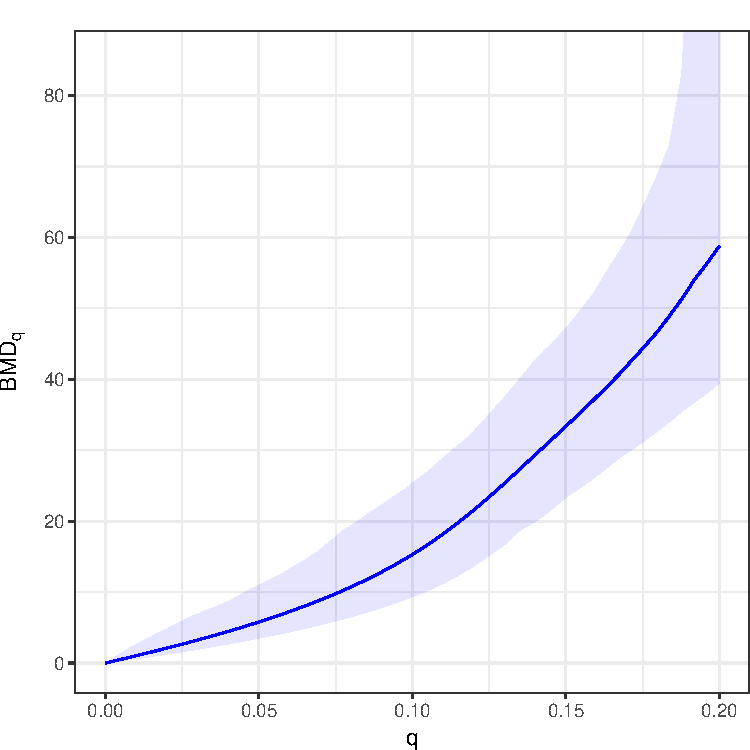
\includegraphics[width=1\textwidth]{cpp_bmd}
\end{minipage}

\begin{minipage}{0.15\textwidth}
\centering(a)
\end{minipage}
%
\begin{minipage}[c]{0.15\textwidth}
\centering(b)
\end{minipage}
%
\begin{minipage}[c]{0.15\textwidth}
\centering (c)
\end{minipage}

\captionof{figure}{Benchmark doses for different values of risk $q$ (a); posterior mean (solid lines), and pointwise 95\% credible bands (shaded areas) for (b)  $R_{\mbox{\textsc{a}}}(x,37)$ and (c) the related BMD$_q$. In the $x$ axis in (b), the observed exposures. }

\end{multicols} 


 %----------------------------------------------------------------------------------------
%	REFERENCES
%----------------------------------------------------------------------------------------
\begin{minipage}[c]{0.85\linewidth}
\bibliographystyle{plainnat}
\bibliography{biblio}
\end{minipage}
\mbox{}
\begin{minipage}[c]{0.15\linewidth}
\centering
Scan the QR code below to download the published paper from Biometrics!

\includegraphics[scale=0.90]{biometrics}
\end{minipage}

\end{document}
